\label{Navegador}
\begin{frame}{Navegador}
    \begin{itemize}
		\item \hyperlink{Contenido}{\beamergotobutton{Contenido}}
		\vspace{1mm}
		\item Ec. Burgers' Determinista. 
		\vspace{1mm}
    	\begin{itemize}
    		\item Galerkin: \hyperlink{Figuras-Galerkin}{\beamergotobutton{Figuras}} \hyperlink{Tablas-Galerkin}{\beamergotobutton{Tablas}}
		    \vspace{1mm}
		    \item \hyperlink{Proyeccion}{\beamergotobutton{Operador Proyeccion}} \hyperlink{Galerkin}{\beamergotobutton{Galerkin}} \hyperlink{Solucion-Galerkin}{\beamergotobutton{Solucion-Galerkin}}
		    \vspace{1mm}
    		\item Colocacion: \hyperlink{Figuras-Colocacion}{\beamergotobutton{Figuras}} \hyperlink{Tablas-Galerkin}{\beamergotobutton{Tablas}}
		    \vspace{1mm}
		    \item \hyperlink{Interpolacion}{\beamergotobutton{Operador Interpolacion}} \hyperlink{Colocacion}{\beamergotobutton{Colocacion}} \hyperlink{Solucion-Colocacion}{\beamergotobutton{Solucion-Colocacion}}
		    \vspace{1mm}
		    \item \hyperlink{Cero-Viscosidad}{\beamergotobutton{Cero-Viscosidad}} \hyperlink{Figuras-Cero-Viscosidad}{\beamergotobutton{Simulaciones}}
		    \vspace{1mm}
    	\end{itemize}
		\vspace{1mm}
		\item Ec. Burgers' Estocastica.
		\begin{itemize}
    		\item \hyperlink{FPK}{\beamergotobutton{Fokker-Planck-Kolmogorov}} 
		    \vspace{1mm}    
    		\item \hyperlink{Figuras-Estocastica}{\beamergotobutton{Figuras}} 
    	\end{itemize}
	\end{itemize}
\end{frame}

%%%% Figuras y Tablas %%%%
%================================
\label{Figuras-Galerkin}
\begin{frame}{Simulaciones: Fourier-Galerkin \hspace{2cm} \hyperlink{Navegador}{\beamergotobutton{Navegador}}}
\begin{figure}
        \centering
        \includegraphics[height=6cm,width=8cm]{files/figures/viscid/galerkin/alphas_Error_N.png}
        \caption{(a) $N = 2^m$, $m = 4, \dots, 12$; $\Delta t = 1.0 \times 10^{-5}$.}
    \end{figure}
\end{frame}

\begin{frame}{Simulaciones: Fourier-Galerkin \hspace{2cm} \hyperlink{Navegador}{\beamergotobutton{Navegador}}}
    \begin{figure}
        \centering
        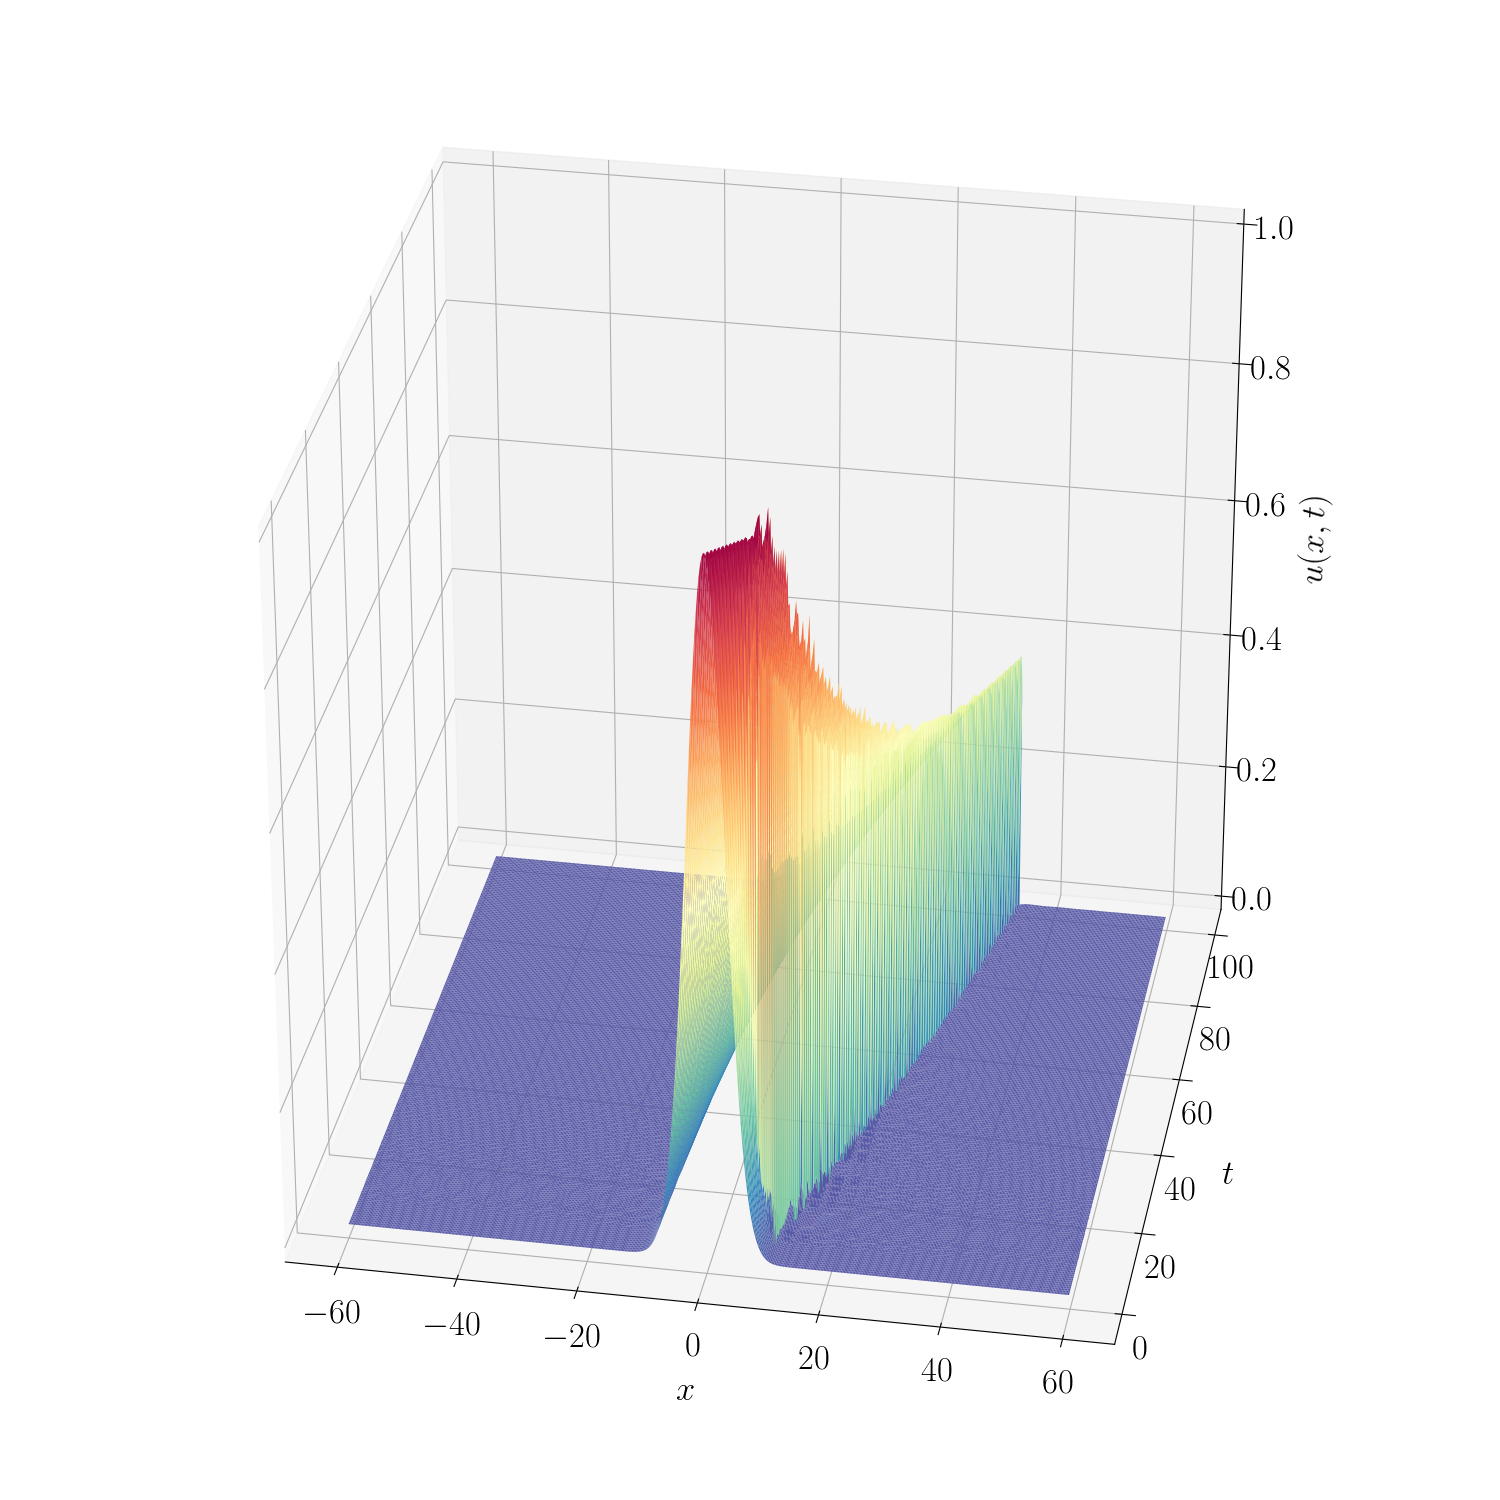
\includegraphics[height=5cm,width=4cm]{files/figures/viscid/galerkin/Numerical_Solution_alpha=0005.png}
        \qquad
        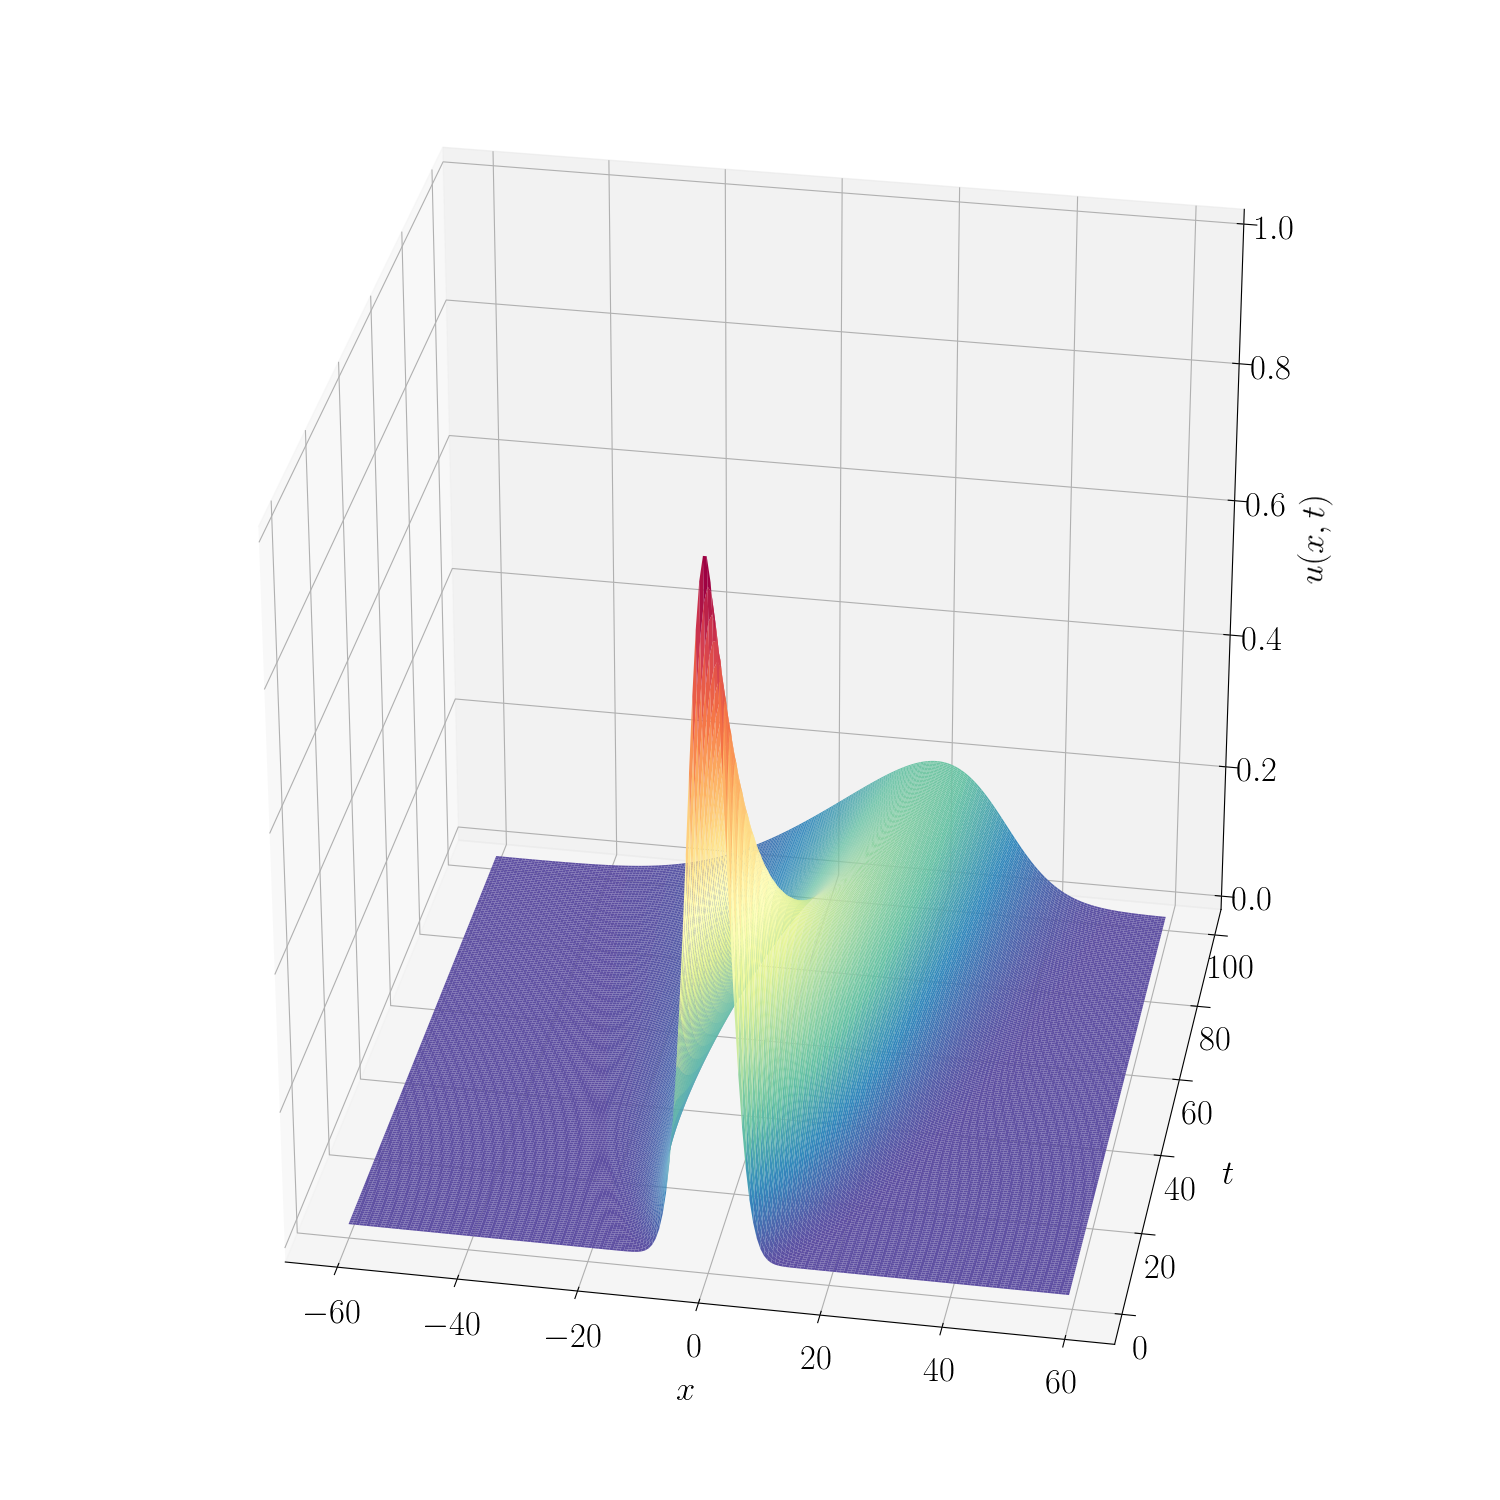
\includegraphics[height=5cm,width=4cm]{files/figures/viscid/galerkin/Numerical_Solution_alpha=1.png}
        \caption{ $\alpha = 0.005$; $N=2048$; $\Delta t = 1.0 \times 10^{-5}$ (b) $\alpha = 1.0$; $N=2048$; $\Delta t = 1.0 \times 10^{-5}$.}
    \end{figure}
\end{frame}

\begin{frame}{Simulaciones: Fourier-Galerkin \hspace{2cm} \hyperlink{Navegador}{\beamergotobutton{Navegador}}}
    \begin{figure}
    	\centering
    	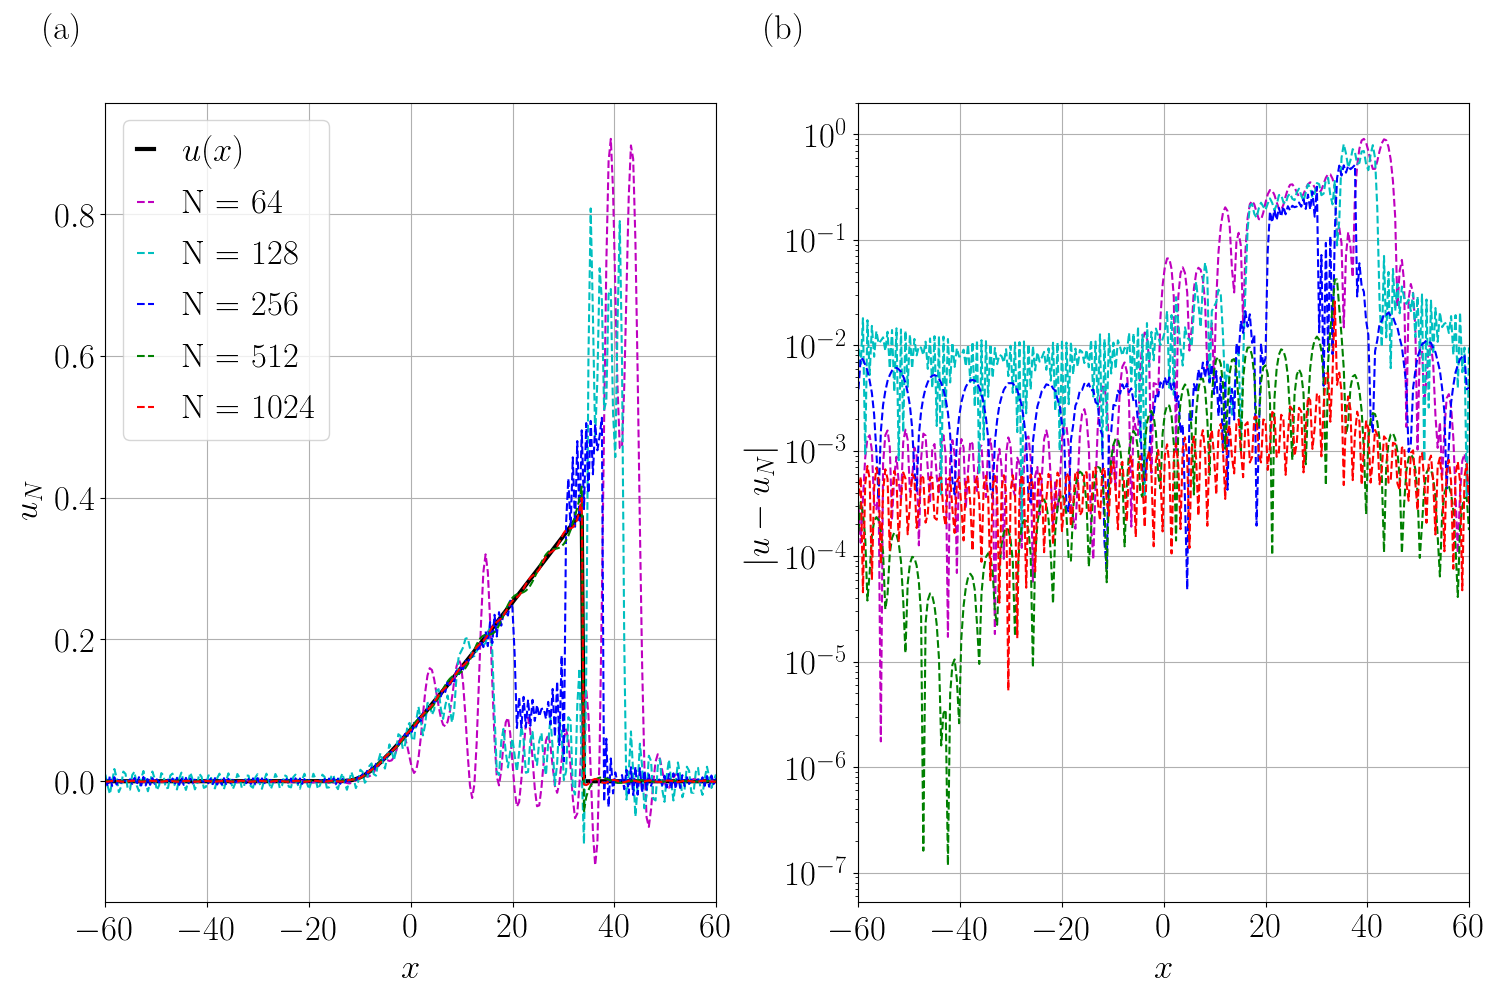
\includegraphics[height=5cm,width=4cm]{files/figures/viscid/galerkin/Numerical_Solution_alpha=0005_T=100.png}
        \qquad
    	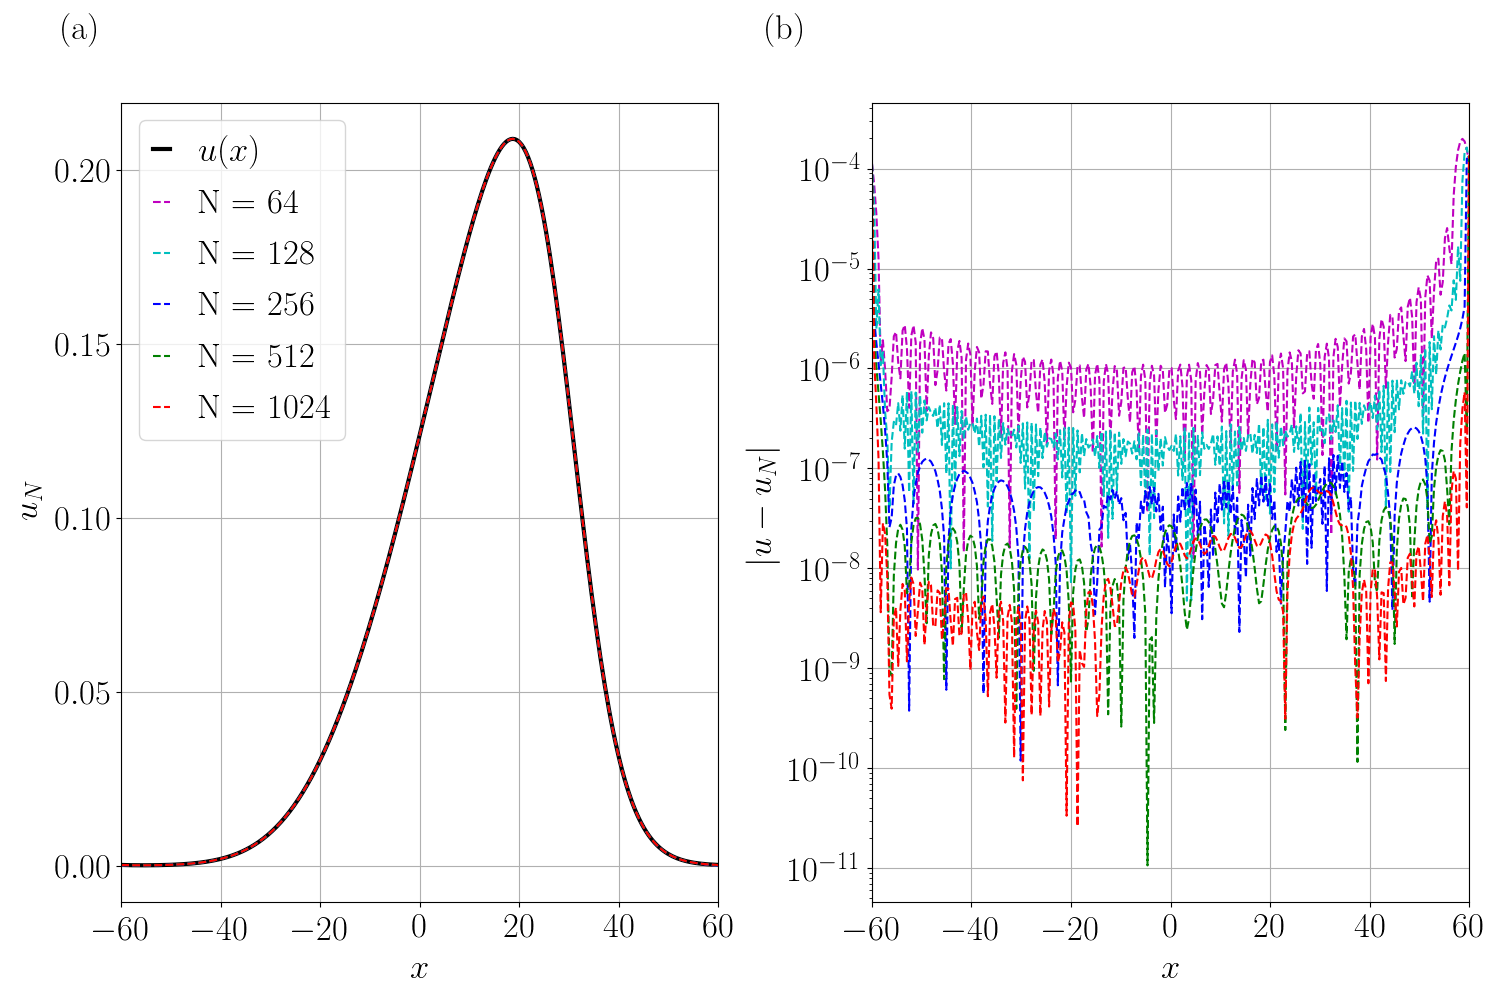
\includegraphics[height=5cm,width=4cm]{files/figures/viscid/galerkin/Numerical_Solution_alpha=1_T=100.png}
        \caption{(a) $t = 100$; $\alpha = 0.005$; $\Delta t = 1.0 \times 10^{-5}$ (b) $t = 100$, $\alpha = 1.0$, $\Delta t = 1.0 \times 10^{-5}$.}
    \end{figure}
\end{frame}

\label{Tablas-Galerkin}
\begin{frame}{Simulaciones: Fourier-Galerkin \hspace{2cm} \hyperlink{Navegador}{\beamergotobutton{Navegador}}}
    \begin{table}
        \centering
        \begin{tabular}{lccc}
        	\toprule
        	\multicolumn{1}{c}{} &\multicolumn{3}{c}{\textbf{Error}} \\
        	N &$\Delta t=1\times 10^{-3}$ &$\Delta t=1\times 10^{-4}$ &$\Delta t=1\times 10^{-5}$ \\
        	\midrule
        	16&0.72504 &0.72504 &0.72504 \\
        	\midrule
        	32& 6.88052 $\times 10 ^{-2}$& 6.87838 $\times 10 ^{-2}$& 6.87816 $\times 10 ^{-2}$ \\
        	\midrule
        	64& 8.85367 $\times 10 ^{-4}$& 8.80521 $\times 10 ^{-4}$& 8.80410 $\times 10 ^{-4}$ \\
        	\midrule
        	128& 9.41793 $\times 10 ^{-5}$& 9.41148 $\times 10 ^{-6}$& 9.41827 $\times 10 ^{-7}$ \\
        	\midrule
        	256& 9.41793 $\times 10 ^{-5}$& 9.41109 $\times 10 ^{-6}$& 9.36411 $\times 10 ^{-7}$ \\
        	\midrule
        	512& 9.41793 $\times 10 ^{-5}$& 9.41109 $\times 10 ^{-6}$& 9.36411 $\times 10 ^{-7}$ \\
        	\bottomrule
        \end{tabular}
        \caption{Error $L_2$}
    \end{table}
\end{frame}

\begin{frame}{Simulaciones: Fourier-Galerkin \hspace{2cm} \hyperlink{Navegador}{\beamergotobutton{Navegador}}}
    \begin{table}
	\centering
	\begin{tabular}{lccc}
		\toprule
		\multicolumn{1}{c}{}& \multicolumn{3}{c}{\textbf{Error}} \\
		$N$& $\Delta t=1\times 10^{-3}$& $\Delta t=1\times 10^{-4}$& $\Delta t=1\times 10^{-5}$ \\
		\midrule
		16& 9.91901& 9.91597& 9.91567 \\
		\midrule
		32& 2.70558& 2.70347& 2.70326 \\
		\midrule
		64& 2.45988& 2.45543& 2.45497 \\
		\midrule
		128& 2.06992& 2.05918& 2.05795 \\
		\midrule
		256& 1.19385& 1.17602& 1.17412 \\
		\midrule
		512& 0.265843& 0.262164& 0.261805 \\
		\midrule
		1024& 0.133743& 0.131882& 0.131699 \\
		\midrule
		2048& 4.70602 $\times 10^{-2}$& 4.57371 $\times 10^{-2}$& 4.56090 $\times 10^{-2}$ \\
		\midrule
		4096& 7.26917 $\times 10^{-3}$& 6.64157 $\times 10^{-3}$& 6.60753 $\times 10^{-3}$ \\
		\bottomrule
	\end{tabular}
	\caption{Error $L_2$}
\end{table}
\end{frame}
%========================
\label{Figuras-Cero-Viscosidad}
\begin{frame}{Simulaciones: Fourier-Galerkin \hspace{2cm} \hyperlink{Navegador}{\beamergotobutton{Navegador}}}
    \begin{figure}
        \centering
        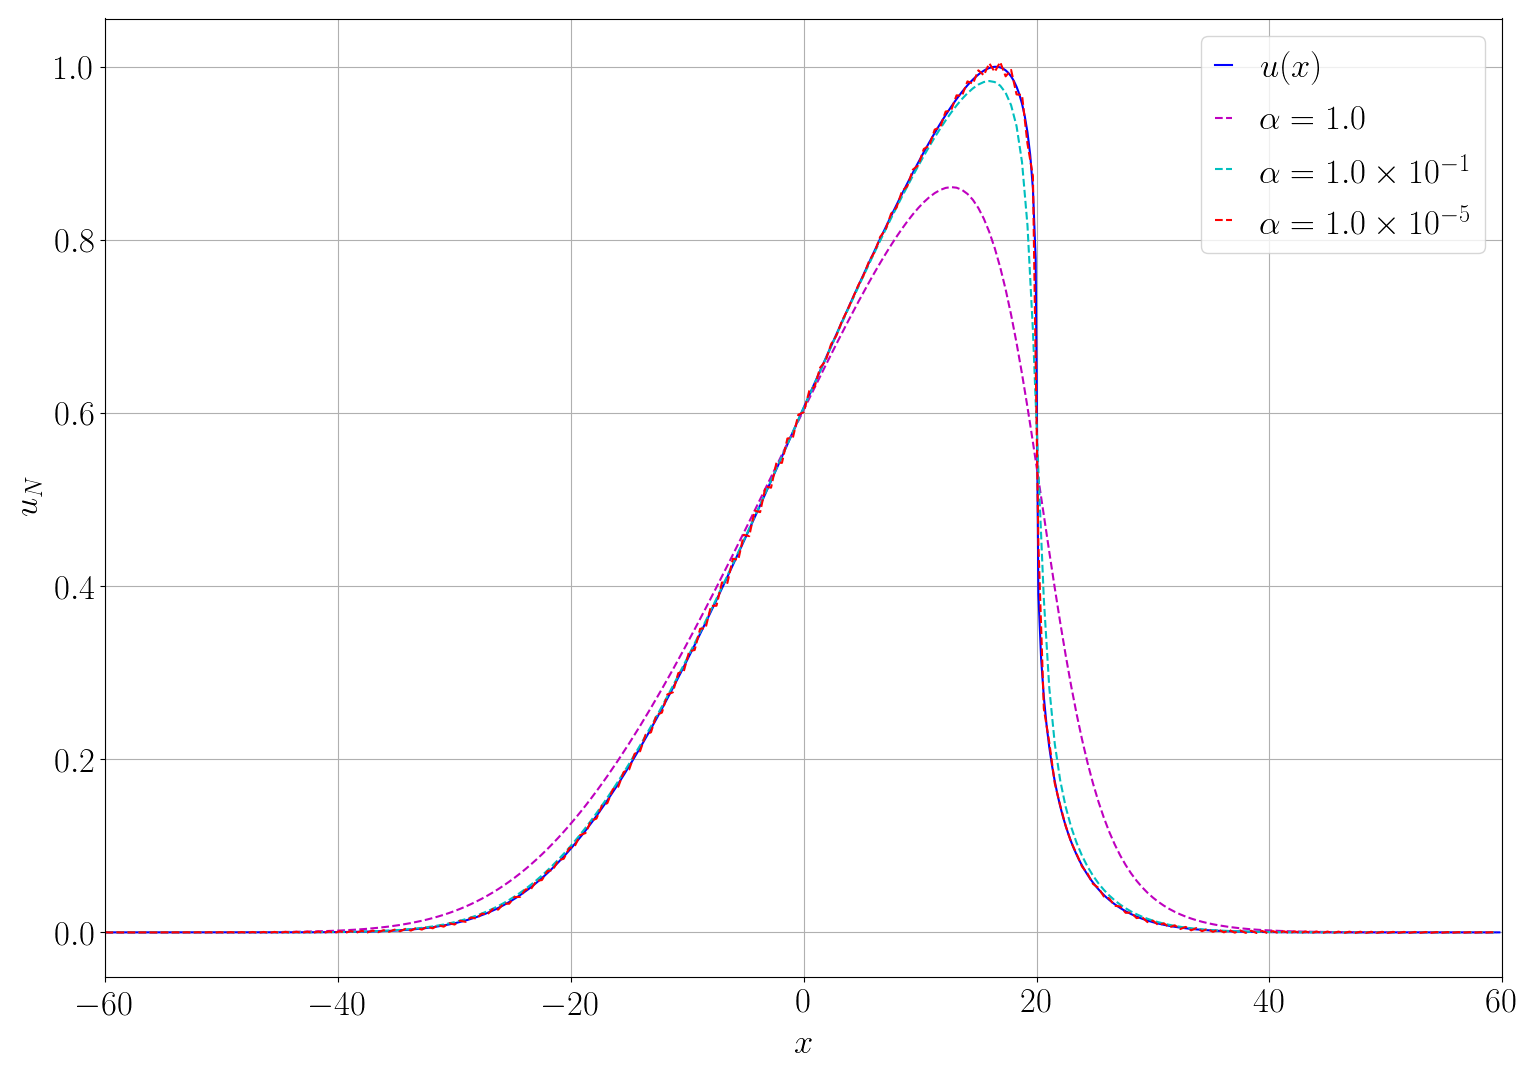
\includegraphics[height=5cm,width=4cm]{files/figures/inviscid/varios_alphas.png}
        \qquad
        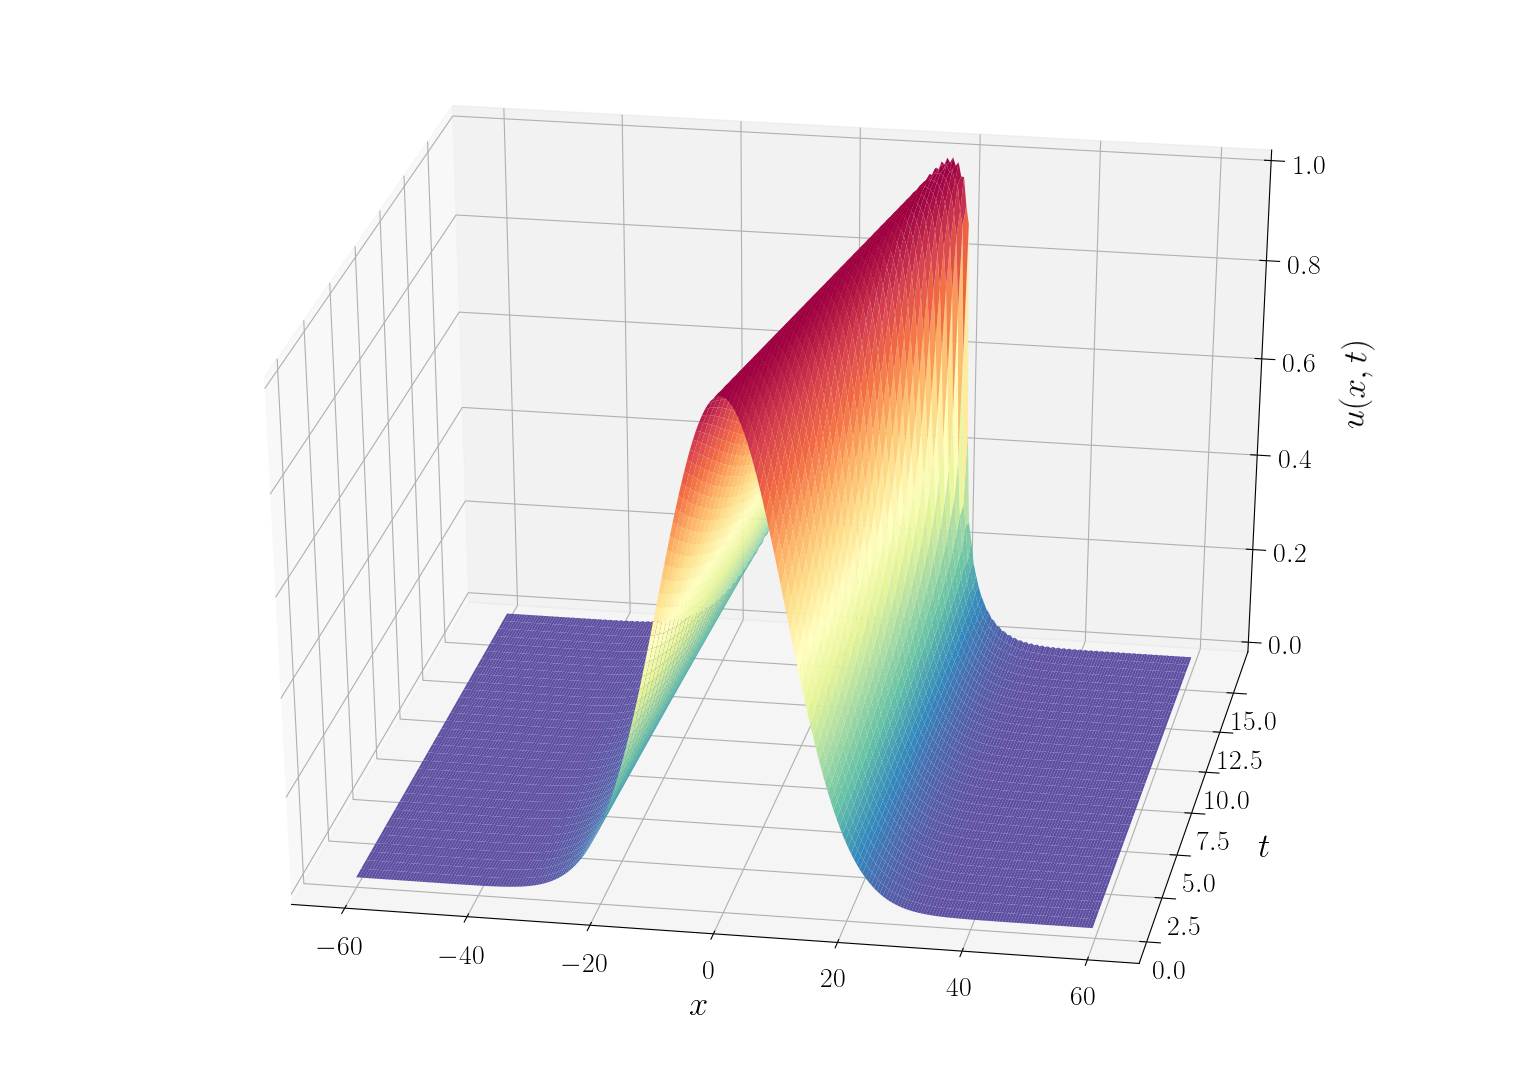
\includegraphics[height=5cm,width=4cm]{files/figures/inviscid/small_alpha.png}
        \caption{(a) $t = T_c, N=256, \Delta t = 1., \times 10^{-3}.$ (b) $\alpha = 1.0, \times 10^{-5}, N=256, \Delta t = 1.0, \times 10^{-3}.$}
    \end{figure}    
\end{frame}

\begin{frame}{Simulaciones: Fourier-Galerkin \hspace{2cm} \hyperlink{Navegador}{\beamergotobutton{Navegador}}}
    \begin{figure}
        \centering
        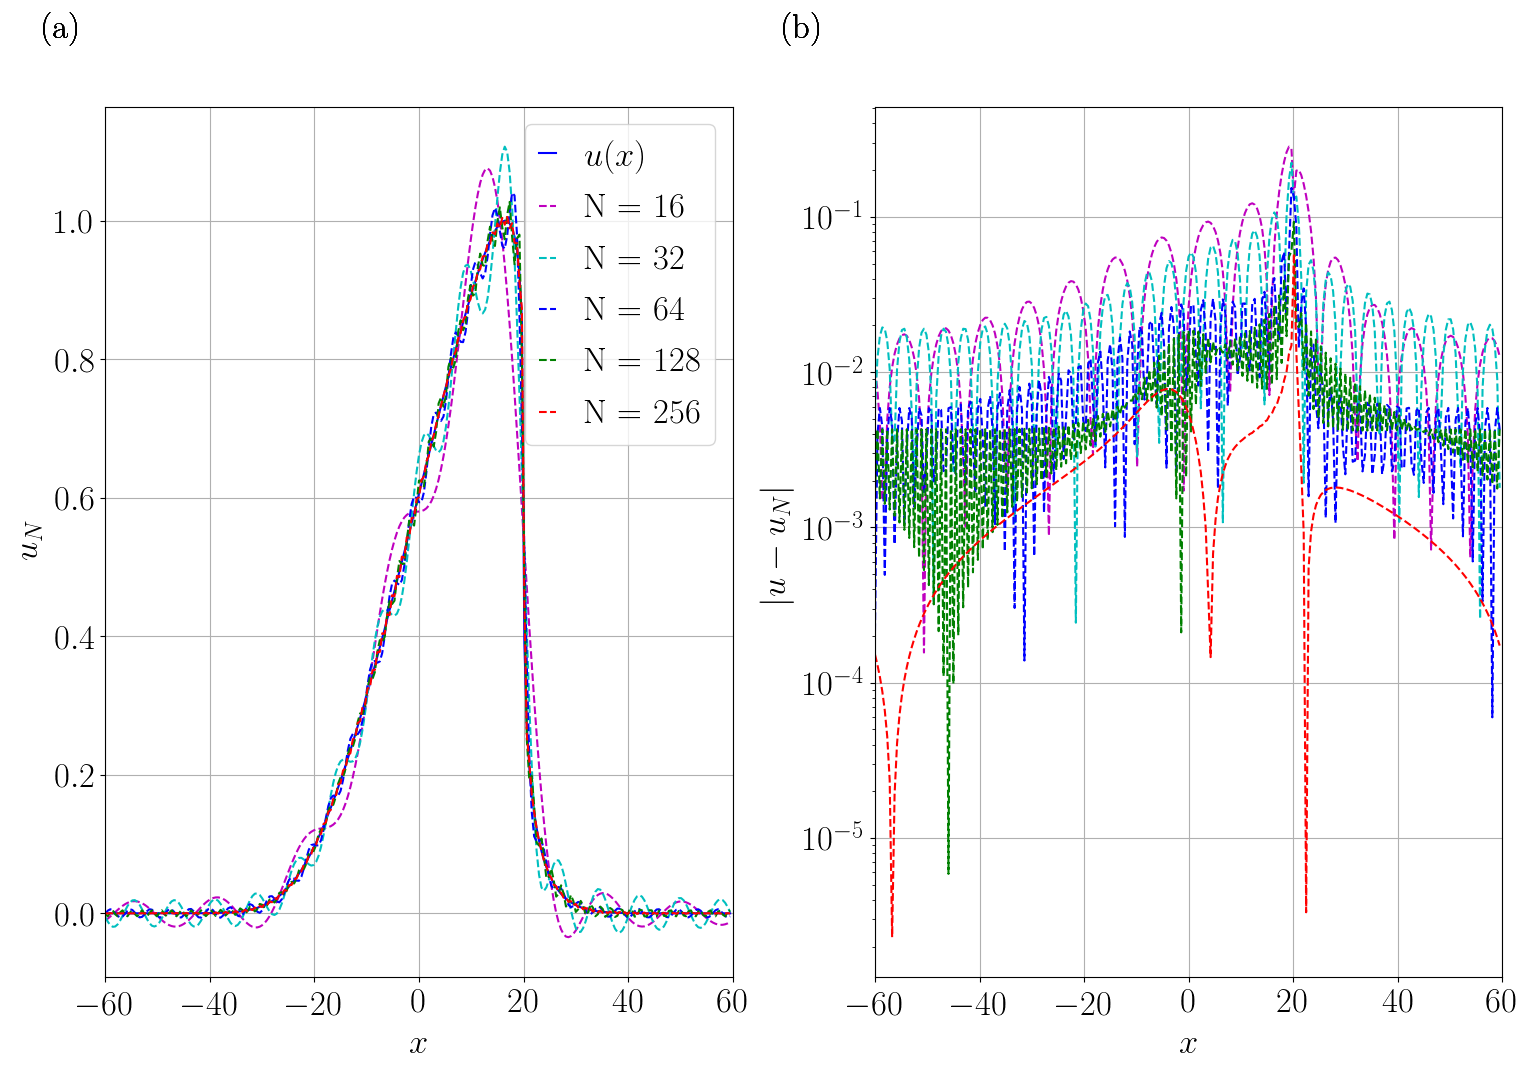
\includegraphics[height=6cm,width=8cm]{files/figures/inviscid/small_alpha_T.png}
        \caption{$t = T_c$; $\alpha = 1.0 \times 10^{-5}$; $\Delta t = 1.0 \times 10^{-3}$}
    \end{figure}
\end{frame}

\begin{frame}{Simulaciones: Fourier-Galerkin \hspace{2cm} \hyperlink{Navegador}{\beamergotobutton{Navegador}}}    
	\begin{table}
		\centering
		\begin{tabular}{lccc}
			\toprule
			\multicolumn{1}{c}{}& \multicolumn{3}{c}{\textbf{Distance}} \\
			$N$& $\Delta t=1\times 10^{-2}$& $\Delta t=1\times 10^{-3}$& $\Delta t=1\times 10^{-4}$ \\
			\midrule
			16& 0.285531& 0.285732& 0.285752 \\
			\midrule
			32& 0.222737& 0.223260& 0.223312 \\
			\midrule
			64& 0.160385& 0.162782& 0.163025 \\
			\midrule
			128& 0.129297& 0.133322& 0.133733 \\
			\midrule
			256& 0.083291& 0.091449& 0.092320 \\
			\bottomrule
		\end{tabular}
		\caption{Error $L_2$}
	\end{table}
\end{frame}
%==========================
\label{Figuras-Colocacion}
\begin{frame}{Simulaciones: Fourier-Colocacion \hspace{2cm} \hyperlink{Navegador}{\beamergotobutton{Navegador}}}
    \begin{figure}
	    \centering
    	\includegraphics[height=6cm,width=10cm]{files/figures/viscid/collocation/alphas_Error_N.png}
    	\caption{$\alpha = 1.0$; $N=2048$; $\Delta t = 1.0 \times 10^{-5}$.}
	\end{figure}
\end{frame}

\begin{frame}{Simulaciones: Fourier-Colocacion \hspace{2cm} \hyperlink{Navegador}{\beamergotobutton{Navegador}}}
	\begin{figure}
	    \centering
    	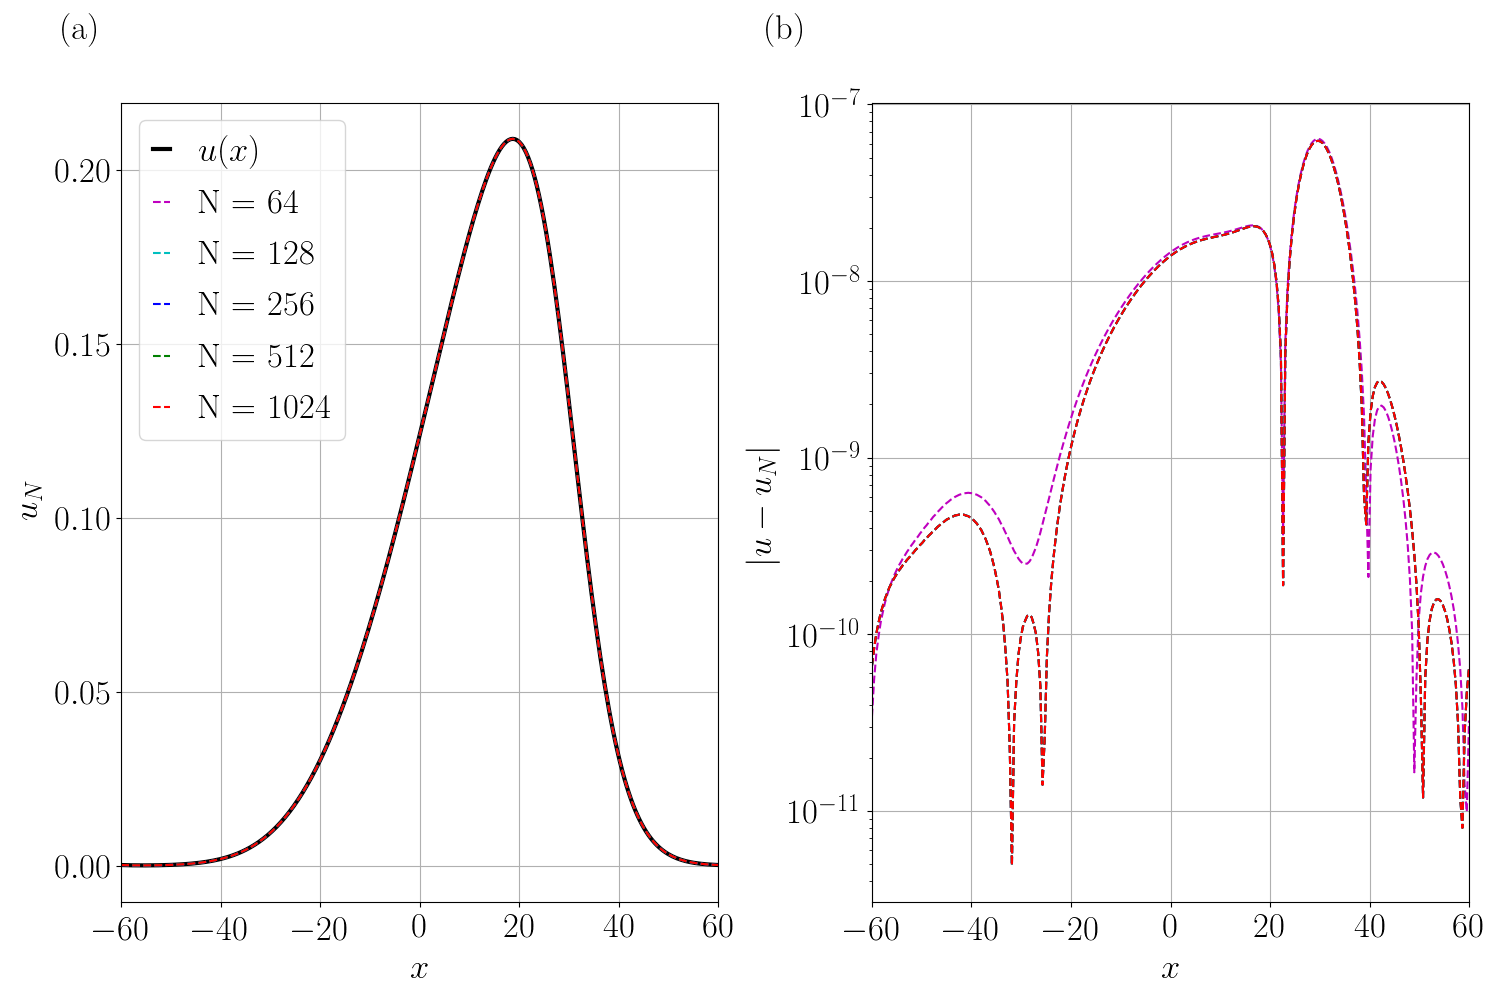
\includegraphics[height=5cm,width=4cm]{files/figures/viscid/collocation/Numerical_Solution_alpha=1_T=100.png}
        \qquad
	    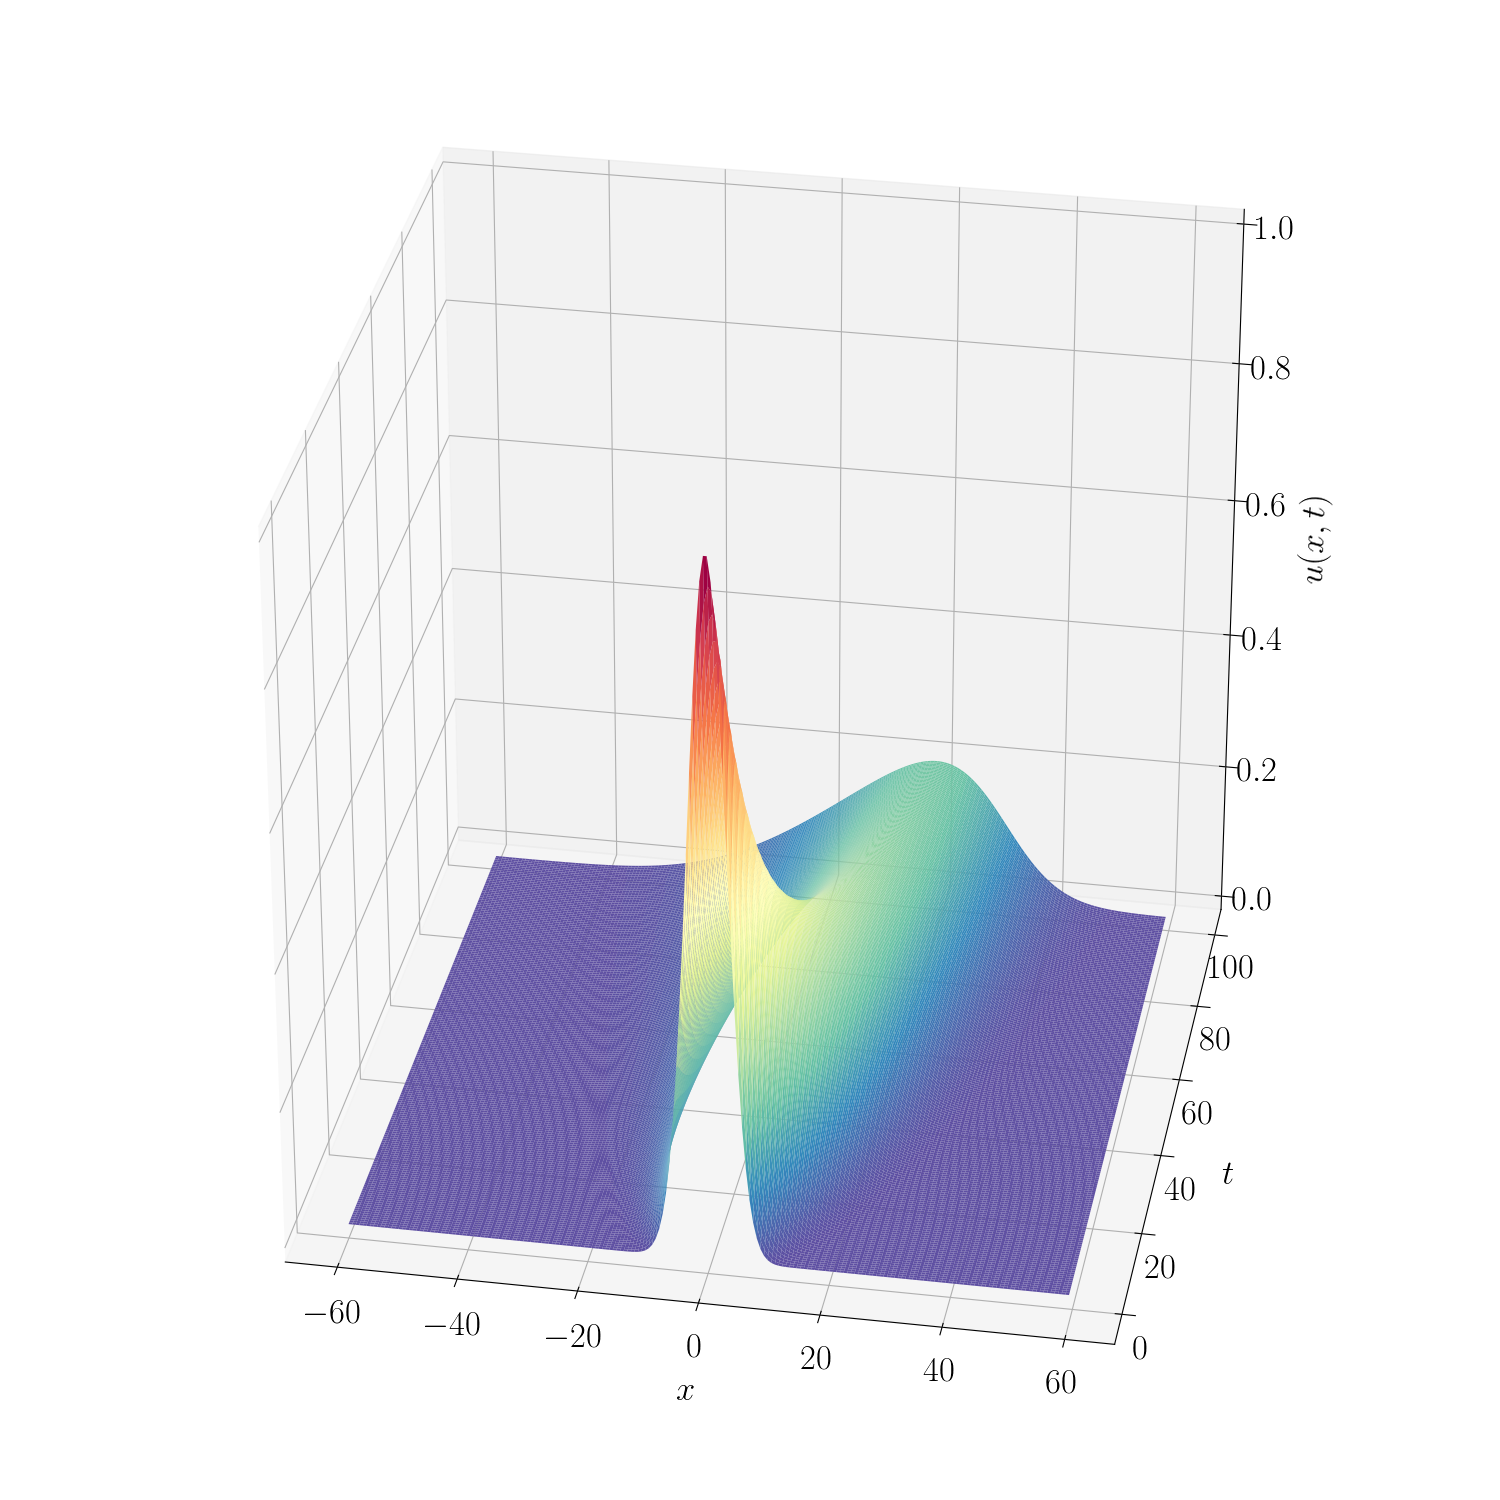
\includegraphics[height=5cm,width=4cm]{files/figures/viscid/collocation/Numerical_Solution_alpha=1.png}
    	\caption{(a) $t = 100$, $\alpha = 1.0$, $\Delta t = 1.0 \times 10^{-5}$. (b) $\alpha = 1.0$; $N=2048$; $\Delta t = 1.0 \times 10^{-5}$.}
	\end{figure}
\end{frame}

\begin{frame}{Simulaciones: Fourier-Colocacion \hspace{2cm} \hyperlink{Navegador}{\beamergotobutton{Navegador}}}
		\begin{figure}
	    \centering
	    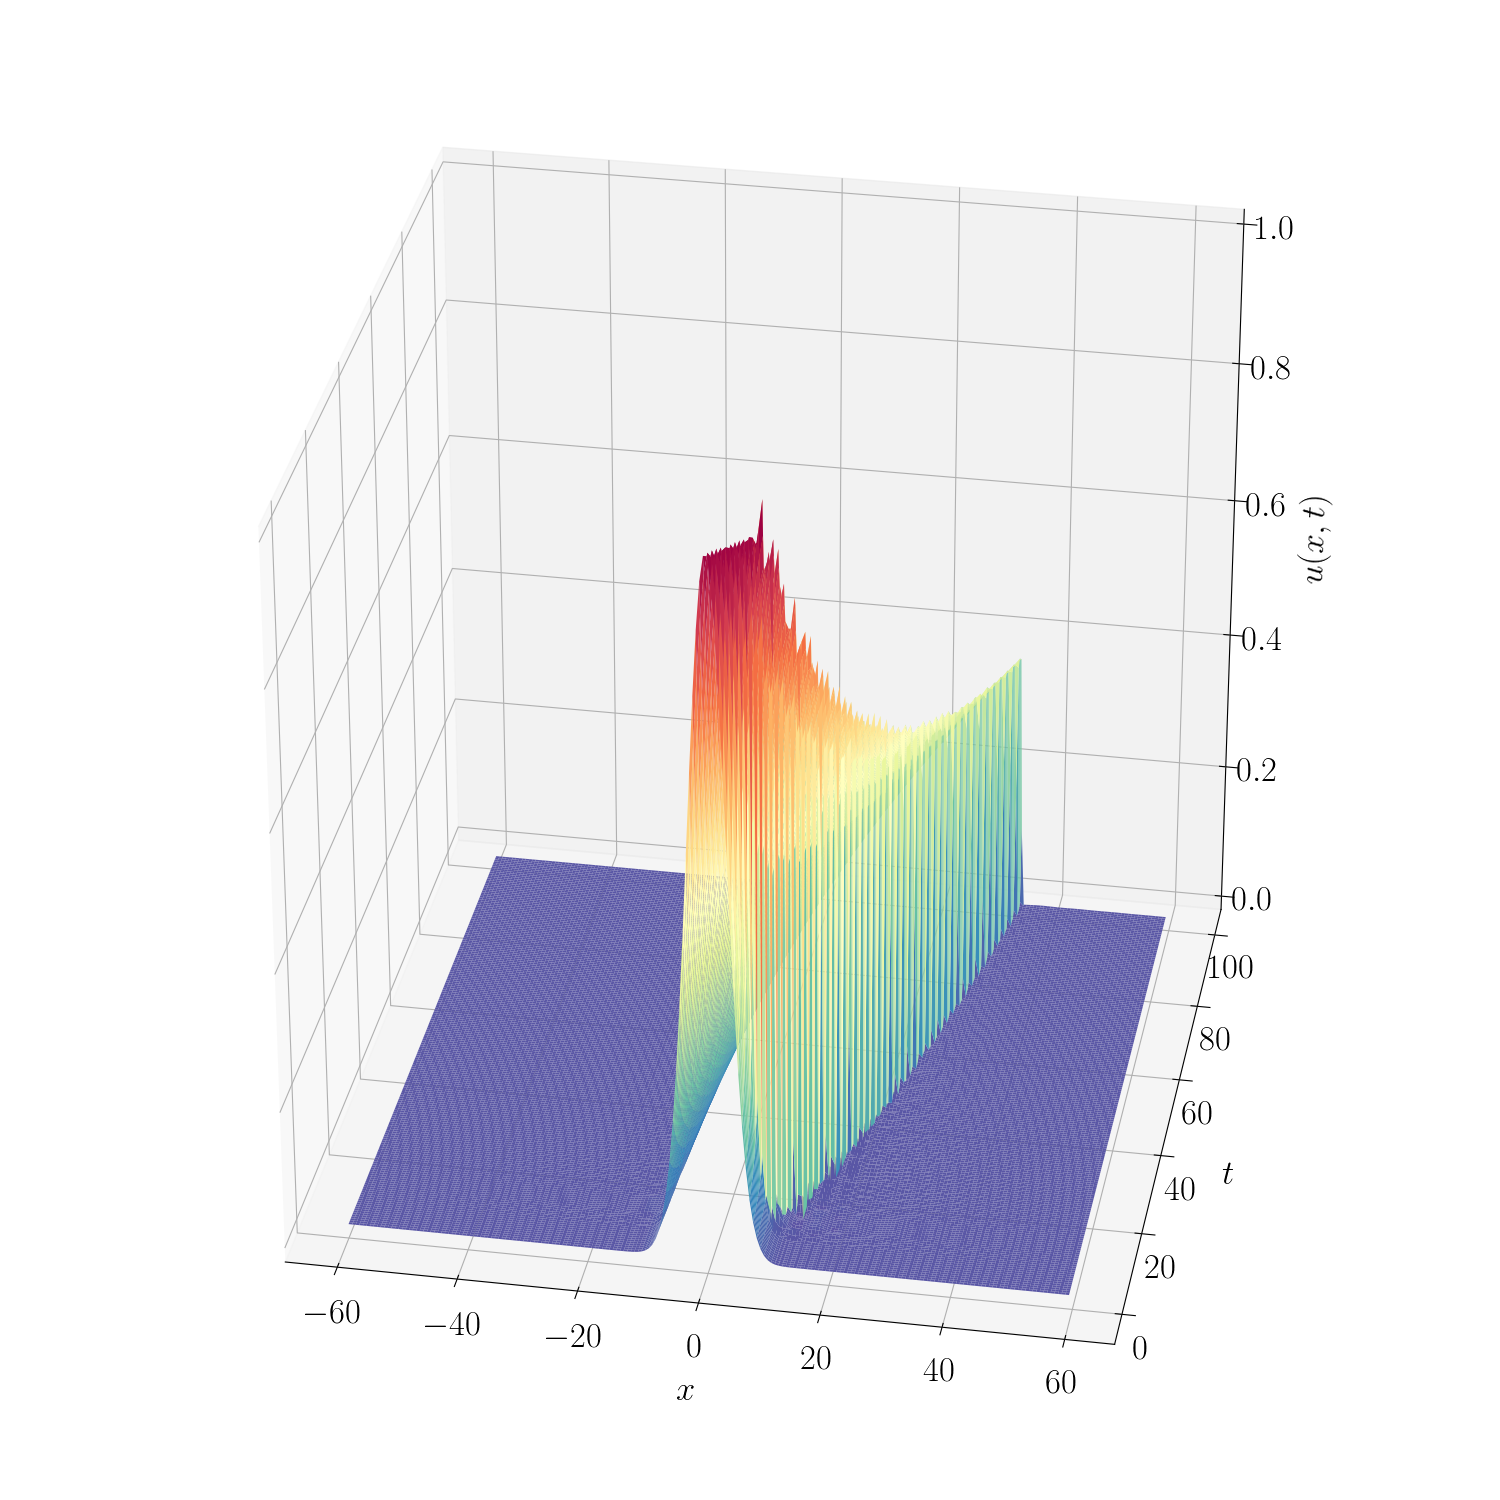
\includegraphics[height=5cm,width=4cm]{files/figures/viscid/collocation/Numerical_Solution_alpha=0005.png}
	    \qquad
	    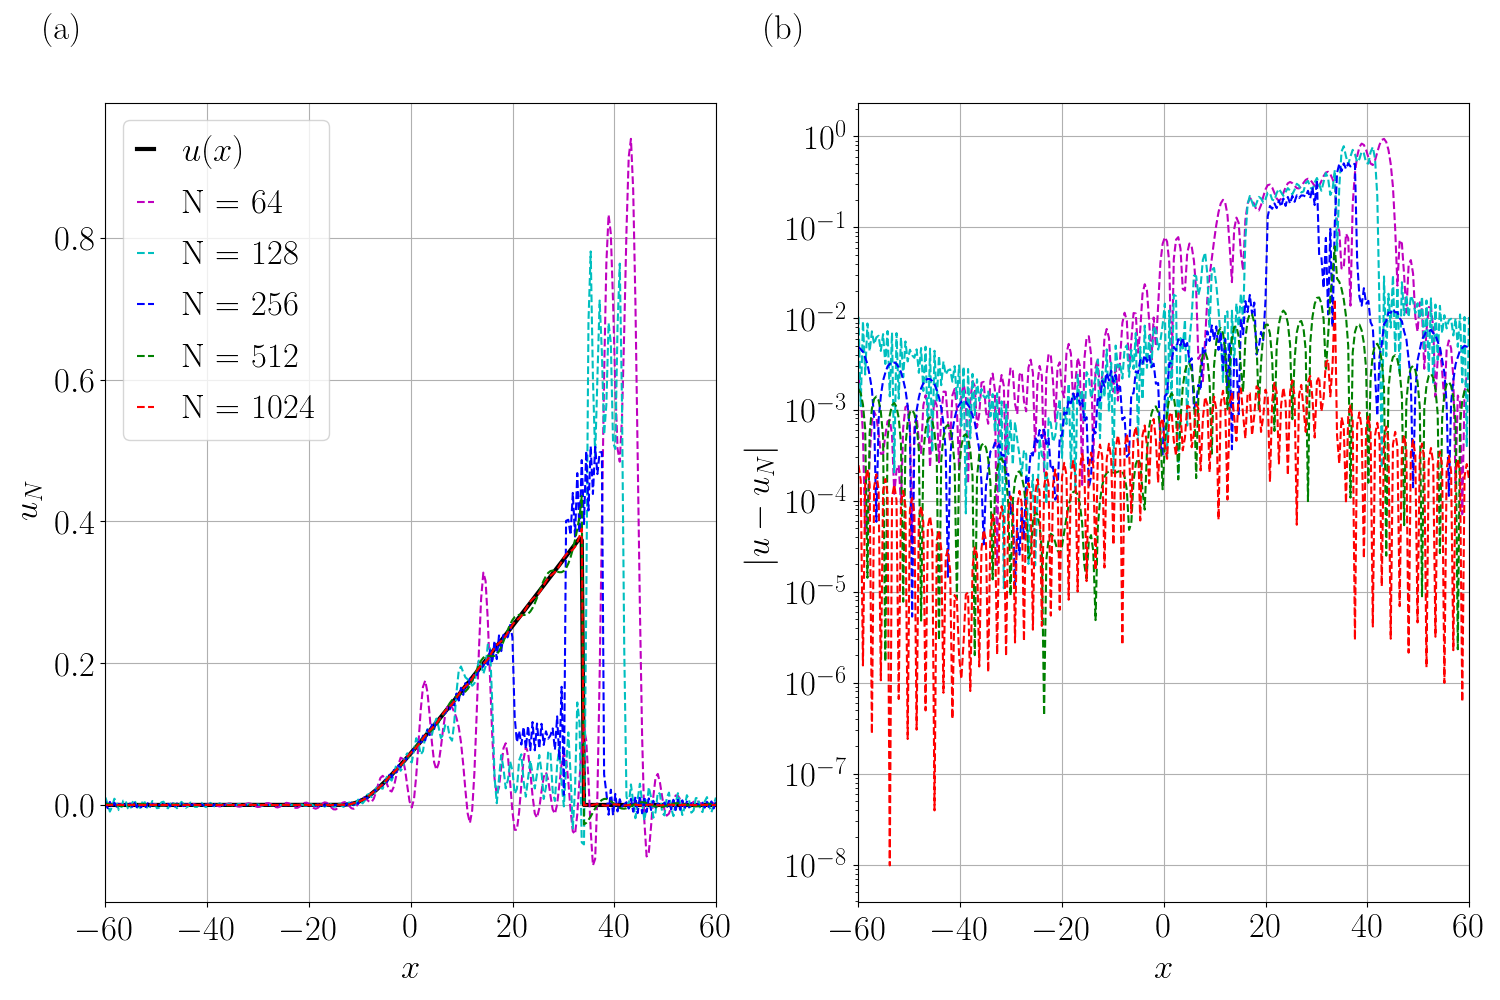
\includegraphics[height=5cm,width=4cm]{files/figures/viscid/collocation/Numerical_Solution_alpha=0005_T=100.png}
    	\caption{(a) $\alpha = 0.005$; $N=2048$; $\Delta t = 1.0 \times 10^{-5}$ (b) $t = 100$, $\alpha = 0.005$, $\Delta t = 1.0 \times 10^{-5}$.}
	\end{figure}
\end{frame}

\label{Tablas-Colocacion}
\begin{frame}{Simulaciones: Fourier-Colocacion \hspace{2cm} \hyperlink{Navegador}{\beamergotobutton{Navegador}}}
	\begin{table}
    \centering
	\begin{tabular}{lccc}
		\toprule
		\multicolumn{1}{c}{}& \multicolumn{3}{c}{\textbf{Error}} \\
		$N$& $\Delta t=1\times 10^{-3}$& $\Delta t=1\times 10^{-4}$& $\Delta t=1\times 10^{-5}$ \\
		\midrule
		16& 0.721112& 0.721112& 0.721112 \\
		\midrule
		32& 4.73004 $\times 10^{-2}$& 4.73015 $\times 10^{-2}$ \\
		\midrule
		64& 7.35344 $\times 10^{-4}$& 7.27561 $\times 10^{-4}$& 7.27283 $\times 10^{-4}$ \\
		\midrule
		128& 1.75152 $\times 10^{-5}$& 1.74583 $\times 10^{-5}$& 1.74574 $\times 10^{-5}$ \\
		\midrule
		256& 1.15509 $\times 10^{-6}$& 1.14669 $\times 10^{-5}$& 1.14659 $\times 10^{-6}$ \\
		\midrule
		512& 9.41793 $\times 10^{-6}$& 7.78847 $\times 10^{-7}$& 7.78707 $\times 10^{-7}$ \\
		\bottomrule
    	\end{tabular}
    	\caption{Error $L_2$}
\end{table}
\end{frame}

\begin{frame}{Simulaciones: Fourier-Colocacion \hspace{2cm} \hyperlink{Navegador}{\beamergotobutton{Navegador}}}
	\begin{table}
    \centering
	\begin{tabular}{lccc}
		\toprule
		\multicolumn{1}{c}{}& \multicolumn{3}{c}{\textbf{Error}} \\
		$N$& $\Delta t=1\times 10^{-3}$& $\Delta t=1\times 10^{-4}$& $\Delta t=1\times 10^{-5}$ \\
		\midrule
		16& 1.35883& 1.35852& 1.35849 \\
		\midrule
		32& 2.65305& 2.65078& 2.65055 \\
		\midrule
		64& 2.45855& 2.45432& 2.45387 \\
		\midrule
		128& 2.0632& 2.05589& 2.05497 \\
		\midrule
		256& 1.18393& 1.16697& 1.16532 \\
		\midrule
		512& 0.304595& 0.300865& 0.300499 \\
		\midrule
		1024& 0.140332& 0.13803& 0.137804 \\
		\midrule
		2048& 4.63808 $\times 10^{-2}$& 4.49226 $\times 10^{-2}$& 4.47813 $\times 10^{-2}$ \\
		\midrule
		4096& 7.66246 $\times 10^{-3}$& 6.9909 $\times 10^{-3}$& 5.4578 $\times 10^{-3}$ \\
		\bottomrule
	\end{tabular}
	\caption{$L_2$}
\end{table}

\end{frame}
%======================
\label{Figuras-Estocastica}
\begin{frame}{Simulaciones: Burgers' Estocastica \hspace{2cm} \hyperlink{Navegador}{\beamergotobutton{Navegador}}}
    \begin{figure}
        \only<1->{
        \centering
        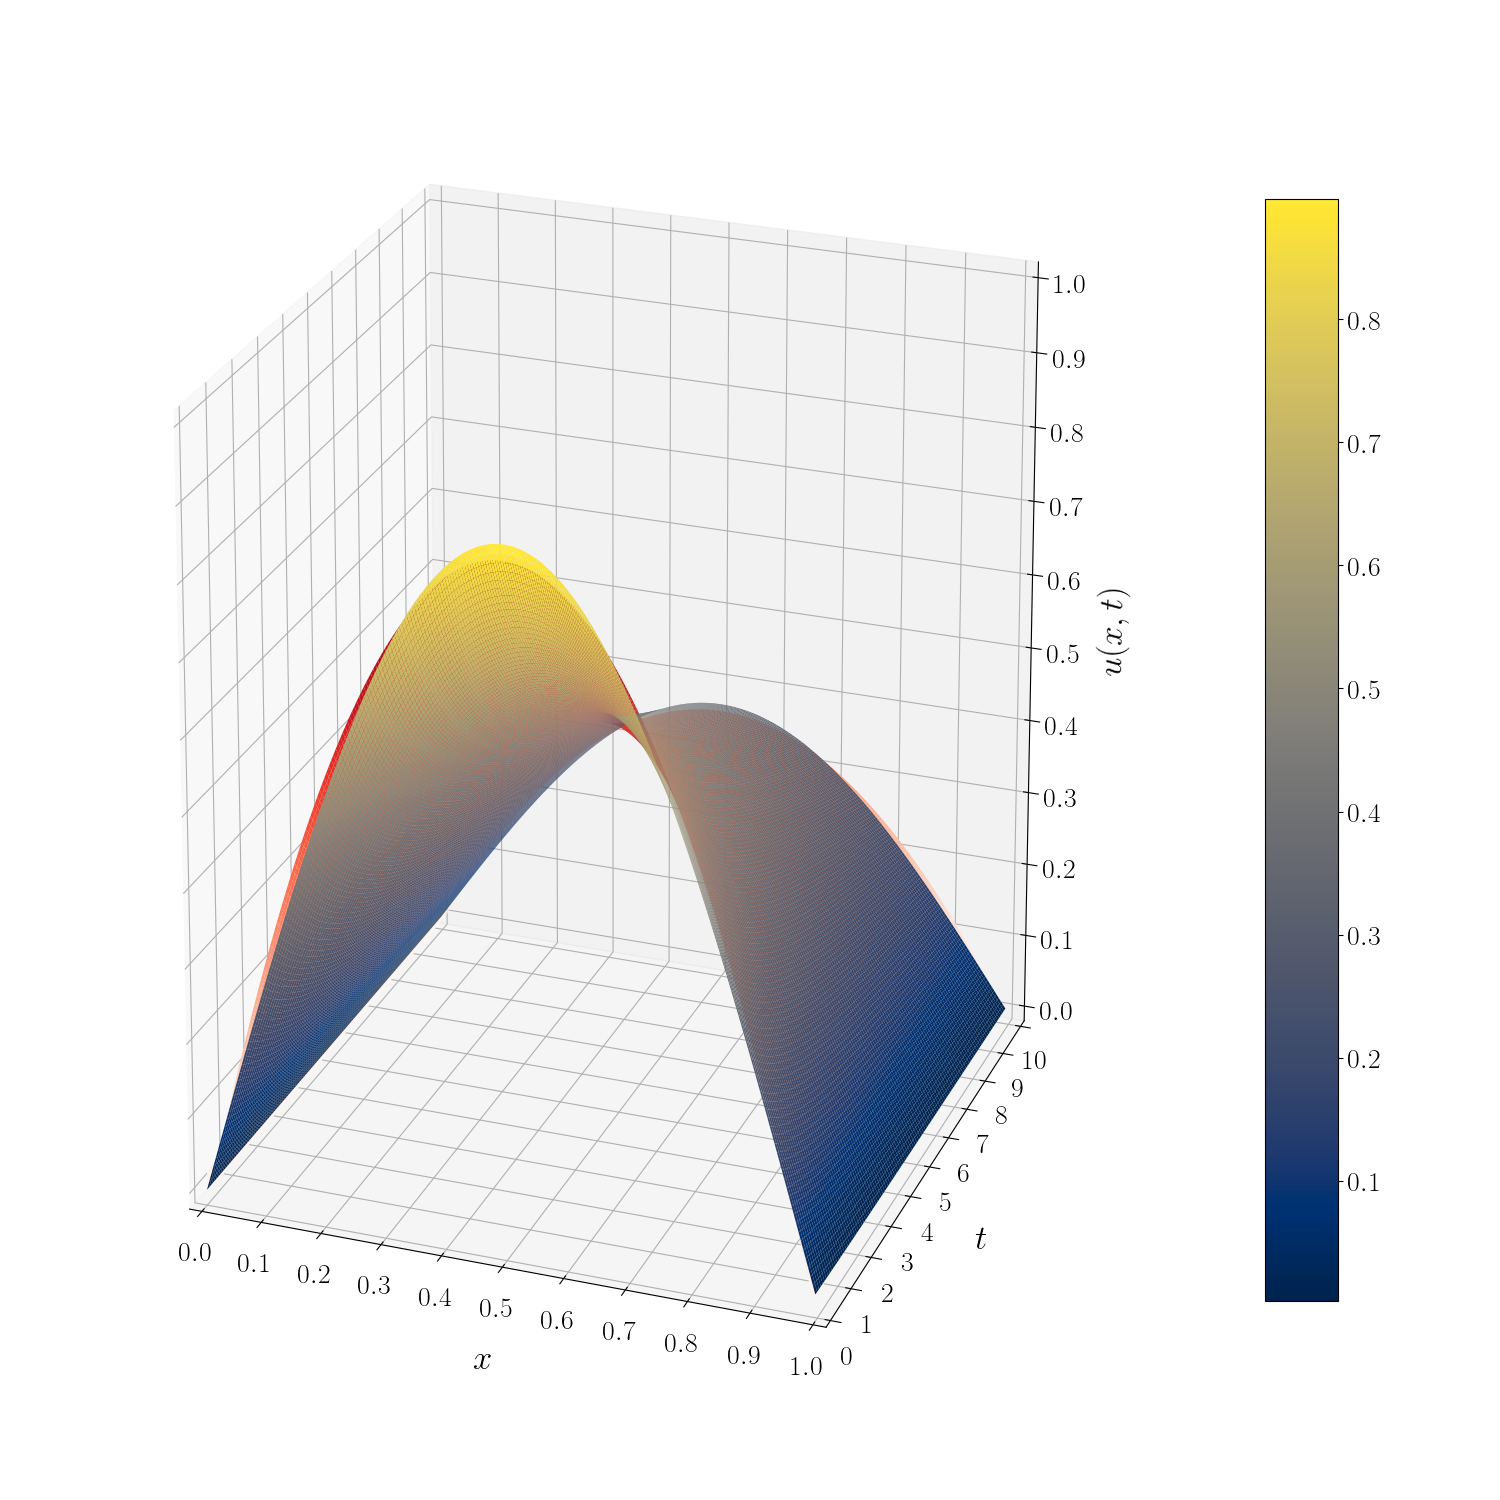
\includegraphics[height=5cm,width=4cm]{files/figures/FPK/Numerical_Solution_Stochastic.png}
	    }
	    \only<2->{
	    \qquad
	    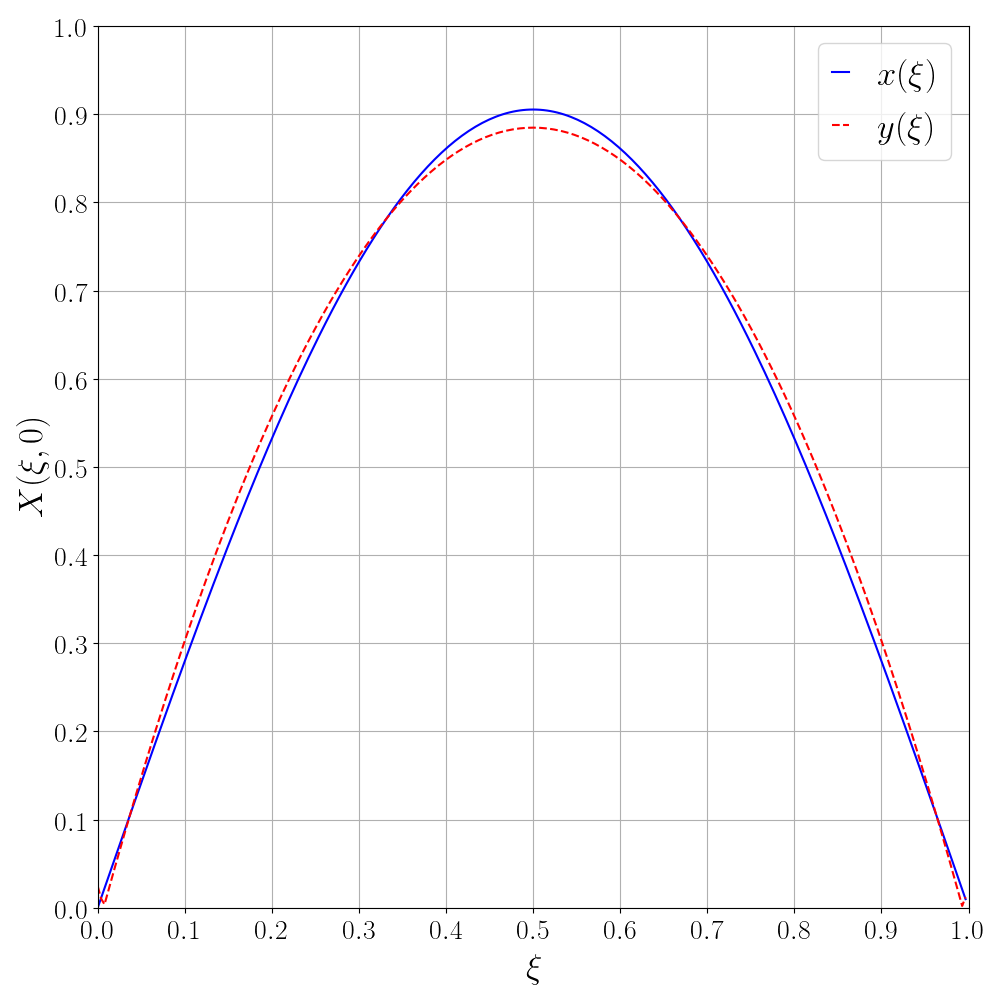
\includegraphics[height=5cm,width=4cm]{files/figures/FPK/IC.png}
    	}
	\end{figure}
\end{frame}

\begin{frame}{Simulaciones: Burgers' Estocastica \hspace{2cm} \hyperlink{Navegador}{\beamergotobutton{Navegador}}}
    \begin{figure}
    \only<1->{
    	\centering
    	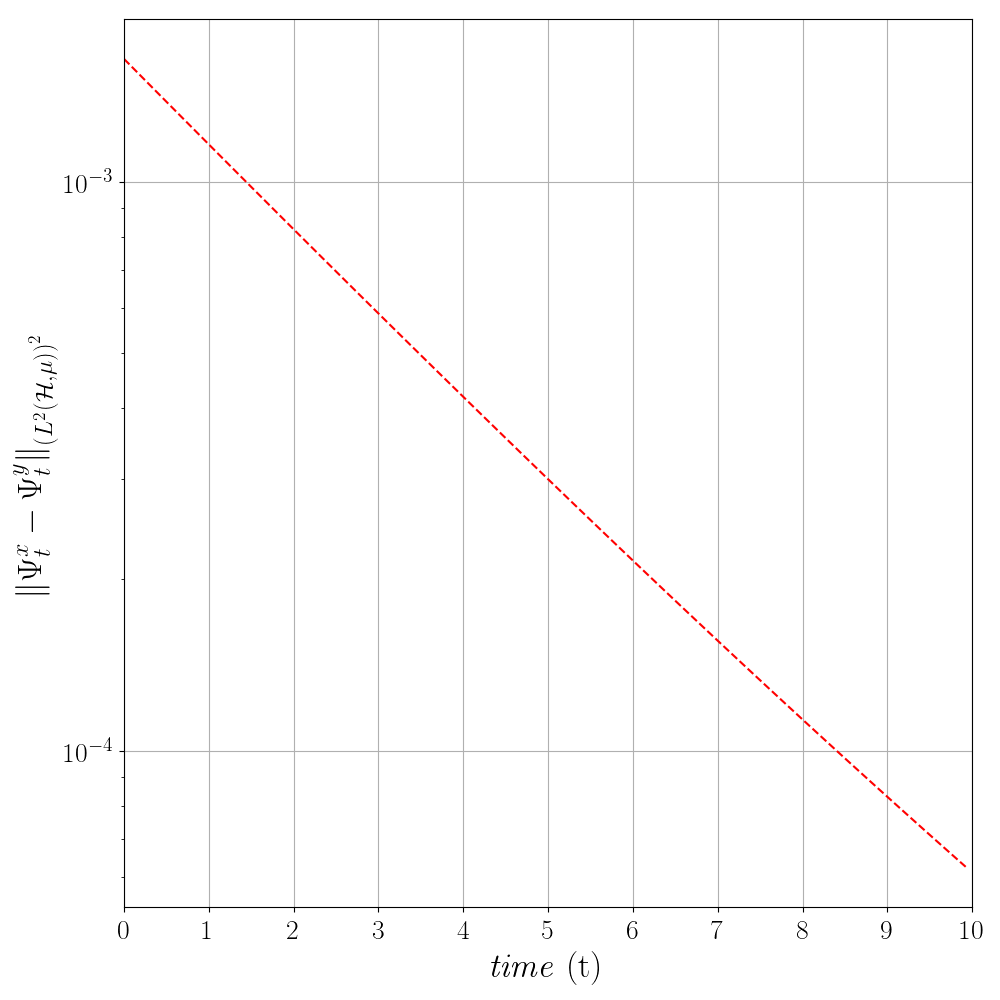
\includegraphics[height=6cm,width=4cm]{files/figures/FPK/norms.png}
    	}
    	\only<2->{
    	\qquad
    	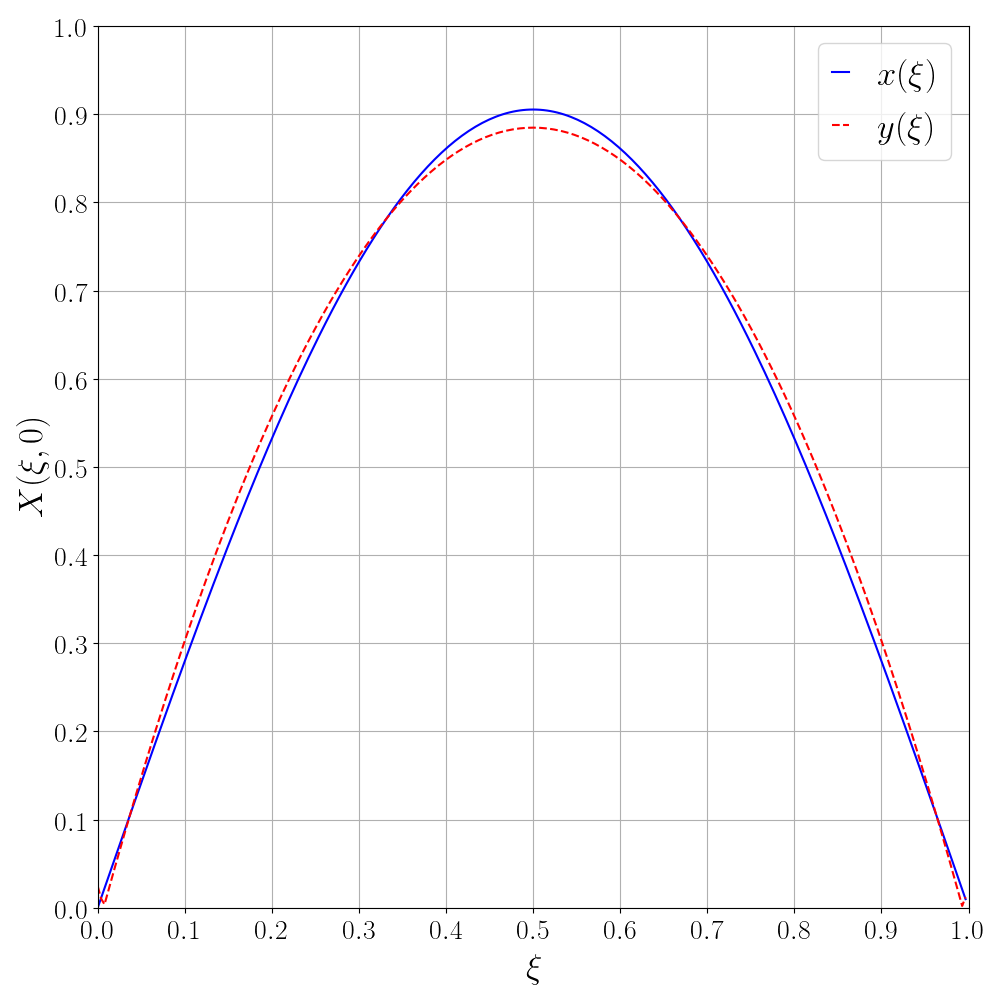
\includegraphics[height=6cm,width=4cm]{files/figures/FPK/IC.png}
    	}
    \end{figure}
\end{frame}	
